\subsection{The lower bound}

\begin{proposition}\label{prop:asym-lower}
$\liminf_{g\downarrow0}g^2N(g)\ge K^2$.
\end{proposition}

\begin{proof}
Fix $\delta\in(0,w/4]$ and $0<g\le g_0(\delta)$, and consider an exit motion with $N$ manoeuvres (\cref{lem:reversal}).
By \cref{lem:confine}, $|\psi|<cg$ on $[0,T_\delta]$.
A parked configuration with $|\psi|<cg$ has $u\le0$: its highest point is at most $H$, and for small $|\psi|$ this forces $u\le\frac w2(1-\cos\psi)-\max(b\sin\psi,-d_b\sin\psi)\le0$.
Let $t_0=\sup\{t\le T_\delta:\ u(t)\le0\}$.
Then $u(t_0)=0$, $0<u\le w-\delta$ on $(t_0,T_\delta]$ and $u(T_\delta)=w-\delta$.

Cut $[t_0,T_\delta]$ into the pieces $I_1,\dots,I_M$ in which it meets the manoeuvres, so $M\le N$.
On $I_j$ the variable $\xi$ is monotone with range at most $1+2Ag+wc$, so by \eqref{eq:lift} the oscillation of $u$ on $I_j$ is at most $Dg^2$ for a constant $D$ (depending on $\delta$).
Put $k_j=\max\big(0,\max_{I_j}u-\tfrac w2\big)\in[0,\tfrac w2-\delta]$.
Then $k_j\ge u-\frac w2$ on $I_j$, so \cref{lem:windows,lem:calib} give
\[
  \Delta_ju\ \le\ g^2\big(r_{k_j}+\Delta_jG_{k_j}\big)+Bg^3 .
\]

Let $F(u)=\int_0^u\dd v/r_*(v)$.
The function $1/r_*=4(R^2-k(u)^2)/R$ is Lipschitz with constant $4w/R$, and on $I_j$ it differs from $1/r_{k_j}$ by at most $(4w/R)Dg^2$.
Hence $F(u_{\rm end})-F(u_{\rm start})\le\Delta_ju/r_{k_j}+(4w/R)D^2g^4$ on every piece.
Using $1/r_{k}\le4R$ we obtain
\[
  F(w-\delta)=\sum_j\big(F(u_{\rm end})-F(u_{\rm start})\big)\ \le\ Mg^2+g^2\sum_j\frac{\Delta_jG_{k_j}}{r_{k_j}}+M\big(4RBg^3+(4w/R)D^2g^4\big).
\]

For the middle sum write $\mathcal H_j=G_{k_j}/r_{k_j}$, and recall that consecutive pieces share their endpoints.
Then
\[
  \sum_j\Delta_j\mathcal H_j=\mathcal H_M(q_{\rm end})-\mathcal H_1(q_{\rm start})+\sum_{j<M}\big(\mathcal H_j-\mathcal H_{j+1}\big)(q_{j+1,\rm start}).
\]
On the bounded set $\{|\phi|<c,\ -Ag-\frac{wc}2\le\xi\le1+Ag+\frac{wc}2\}$, which contains all states on $[t_0,T_\delta]$, the functions $G_k/r_k$ are bounded by a constant $\hat H$ and are Lipschitz in $k$ with constant $E$ (both depending on $\delta$).
Moreover $|k_j-k_{j+1}|\le2Dg^2$.
Hence $\sum_j\Delta_j\mathcal H_j\le2\hat H+2EDg^2M$.
Altogether
\[
  F(w-\delta)\ \le\ Mg^2\big(1+O(g)\big)+2\hat Hg^2,
\]
so $\liminf_{g\to0}g^2N(g)\ge F(w-\delta)$.
Letting $\delta\to0$ gives $\liminf g^2N(g)\ge F(w)=K^2$.
\end{proof}

\subsection{The construction: tilted S-curves}\label{sec:construction}

For $u\ge0$ let $k(u)=\min\big(\max(0,u-\tfrac w2),\tfrac w2\big)$, $s_\pm=s_\pm(k(u))$, and define the \emph{tilt}
\[
  \varpi(u)=\frac{s_--s_+}2=\frac{k}{R^2-k^2}.
\]
Fix $\lambda\in(0,1)$.
The \emph{ideal loop} at height $u$ is the closed curve in the $(\zeta,\phi)$-plane, $\zeta=\zeta_{k(u)}$, through the cusps
\[
  \mathcal A_u=\Big(\frac{1-\lambda}2,\ \frac{\lambda\varpi}2\Big),\qquad \mathcal B_u=\Big(\frac{1+\lambda}2,\ -\frac{\lambda\varpi}2\Big).
\]
Its upper branch runs from $\mathcal A_u$ with slope $s_+$ and then with slope $-s_-$ to $\mathcal B_u$.
Its lower branch runs from $\mathcal A_u$ with slope $-s_-$ and then with slope $s_+$ to $\mathcal B_u$.

\begin{lemma}\label{lem:loop}
The ideal loop has area $2\lambda^2r_*(u)$.
It lies in the homothetic image $\lambda\Pi_u$ of the window of \cref{rem:parallelogram} under the homothety of ratio $\lambda$ about $(\frac12,0)$, hence at distance at least $(1-\lambda)\varrho_0$ from $\partial\Pi_u$.
Here $\varrho_0>0$ does not depend on $u\in[0,w]$.
\end{lemma}

\begin{proof}
For $\lambda=1$ the loop is the parallelogram with vertices $\mathcal A_u=(0,\frac\varpi2)$, $\mathcal B_u=(1,-\frac\varpi2)$ and the turning points $\mathcal U=(\frac12,\frac{s_++s_-}4)$, $\mathcal D=(\frac12,-\frac{s_++s_-}4)$.
(With $\varpi=(s_--s_+)/2$ both turning points have abscissa $\frac12$.)
Its area is $\frac12\cdot1\cdot\frac{s_++s_-}2=\frac{s_++s_-}4=2r_*(u)$.
For general $\lambda$ the loop is the image under the homothety of ratio $\lambda$ about $(\frac12,0)$, so the area scales by $\lambda^2$.

Next we check that the four vertices lie in the convex set $\Pi_u$; then so does the whole loop.
For $u\le w/2$ (so $k=0$, $\varpi=0$) the vertices are $(0,0)$, $(1,0)$, $(\frac12,\pm\frac1{2R})$.
They satisfy $\frac w2|\phi|\le\xi\le1-\frac w2|\phi|$ because $\frac w{4R}<\frac12$, and this rhombus, with vertices $(0,0)$, $(1,0)$, $(\frac12,\pm\frac1w)$, is contained in $\Pi_u$.
For $u\ge w/2$, with $k=u-\frac w2\in[0,\frac w2]$ and $w-u=\frac w2-k$:
\begin{itemize}[nosep]
\item $\mathcal A_u$ and $\mathcal B_u$ lie on the sides $\zeta=0,1$, and they satisfy $0\le\zeta+(w-u)\phi\le1$ because $(w-u)\frac\varpi2\le1$.
The latter is equivalent to $k(\frac w2-k)\le2(R^2-k^2)$, i.e.\ to $k^2+\frac{kw}2\le2R^2$, which holds since $k^2+\frac{kw}2\le\frac{w^2}2<2R^2$ for $k\le\frac w2<R$.
\item $\mathcal U$ and $\mathcal D$ satisfy $0\le\frac12\pm(w-u)\frac{s_++s_-}4\le1$ because $(w-u)(s_++s_-)\le2$.
This is equivalent to $(\frac w2-k)R\le R^2-k^2=(R-k)(R+k)$, which holds since $\frac w2-k\le R-k$ and $R\le R+k$.
\end{itemize}
Finally, $\Pi_u$ contains a disk of radius $\varrho_0>0$ about $(\frac12,0)$, with $\varrho_0$ independent of $u\in[0,w]$ (its sides stay at distance bounded below from that point).
The homothety therefore maps $\Pi_u$ into the set of points at distance at least $(1-\lambda)\varrho_0$ from $\partial\Pi_u$.
\end{proof}

The ideal loop is realised by two manoeuvres, each consisting of two full-lock arcs (an S-curve).
\begin{itemize}[nosep]
\item Forward: full left lock, then full right lock; this follows the upper branch from $\mathcal A_u$ to $\mathcal B_u$.
\item Reverse: full left lock, then full right lock; in reverse the heading first decreases and then increases, so this follows the lower branch back to $\mathcal A_{u'}$, where $u'$ is the new height.
\end{itemize}
Explicitly, a forward S-curve from heading $\psi_A$ to heading $\psi_B$ with horizontal displacement $\Delta x$ has its apex heading $\psi_{\rm top}$ given by $2\sin\psi_{\rm top}=\Delta x/R+\sin\psi_A+\sin\psi_B$.
It lifts the car by $R\big(\cos\psi_A+\cos\psi_B-2\cos\psi_{\rm top}\big)$.
The reverse S-curve is analogous, with apex heading $\psi_{\rm bot}$.

\begin{proposition}\label{prop:asym-upper}
$\limsup_{g\downarrow0}g^2N(g)\le K^2$.
\end{proposition}

\begin{proof}
Fix $\lambda\in(0,1)$.
Start from the parked level configuration $q_0=\big((d_b+g\frac{1-\lambda}2,\ m+\frac w2),0\big)$, at height $u=0$ with $(\zeta,\phi)=\mathcal A_0$.
Repeat \emph{cycles}: from the configuration corresponding to $\mathcal A_u$ at height $u$, drive the forward S-curve to the configuration corresponding to $\mathcal B_u$.
Then drive the reverse S-curve to the configuration corresponding to $\mathcal A_{u_1}$, where $u_1$ is the height reached after the forward S-curve; the reverse S-curve changes the height only by $O(g^2)$.

\emph{Feasibility.}
In rescaled coordinates the arcs of an S-curve have slope $\dd\phi/\dd\zeta=s_+(1+O(g^2))$ and $-s_-(1+O(g^2))$.
The S-curve is determined by its end points through the explicit formula for its apex heading above, which depends continuously on the data. Its rescaled trace consists of two curves of slopes $s_+(1+O(g^2))$ and $-s_-(1+O(g^2))$ joining the same end points as the two segments of the ideal branch, so the turning points differ by $O(g^2)$ and the trace lies within $O(g^2)$ of the ideal branch, uniformly in $u$. The reverse S-curve is aimed at the cusp $\mathcal A_{u_1}$; since $|u_1-u|=O(g^2)$, this differs from $\mathcal A_u$ by $O(g^2)$, which the same estimates absorb.
Next we need \emph{sufficient} conditions for freeness.
Here $c$ denotes a constant larger than the largest $|\phi|$ on the loops, $(s_++s_-)/4$ (it is not the constant of \cref{lem:confine}).
Let $|\psi|<cg$ and $u\ge A''g$, where $A''=2c(b+d_b)$.
Then no point of the car lies at height $\le m$, and the curb is no issue.
The part of the footprint inside the band $(m,H)$ has its leftmost and rightmost points among the corners and the points where the front and rear edges cross the line $y=H$.
Hence $q$ is free if, for $\psi\ge0$,
\begin{align*}
  P_x&\ge d_b\sec\psi+(\tfrac w2-u)\tan\psi &&\text{if }\cRL_y\ge H,\\
  P_x&\ge d_b\cos\psi+\tfrac w2\sin\psi &&\text{if }\cRL_y<H,\\
  P_x&\le L-b\cos\psi-\tfrac w2\sin\psi ,
\end{align*}
and symmetrically for $\psi<0$.
The last condition is still sufficient when $\cFC$ lies above $H$, since the band part then ends at the crossing of the curb-side edge with $y=H$, to the left of $\cFC$.
For $u\ge A''g$ the corner $\cRL$ (for $\psi\ge0$) or $\cFL$ (for $\psi<0$) lies above $H$.
So, in rescaled coordinates and up to $O(g)$, these conditions are exactly the constraints defining $\Pi_u$; for $u<w/2$ we use $k=0$ and the second parallelogram of \cref{rem:parallelogram}.
Thus the set of free rescaled states contains $\{(\zeta,\phi):\mathrm{dist}((\zeta,\phi),\R^2\setminus\Pi_u)\ge A'g\}$ for a constant $A'$.
For $0\le u<A''g$ we use instead the conservative sufficient condition that the whole footprint lies in $\{0\le x\le L\}$; the curb is again no issue, because the lowest point is at height at least $m-O(g)>0$.
In rescaled coordinates this reads $\tfrac w2|\phi|+O(g)\le\xi\le1-\tfrac w2|\phi|-O(g)$, and the untilted loop satisfies it with margin $\frac{1-\lambda}2(1-\frac w{2R})$.
By \cref{lem:loop} all cycles are therefore free once $g$ is small enough (depending on $\lambda$).

\emph{Lift per cycle.}
By \eqref{eq:lift}, the lift of a manoeuvre is $g^2\big(\int\phi\,\dd\xi+O(g^2)\big)$.
Over a cycle this is $g^2$ times the area enclosed by the rescaled trace in the $(\xi,\phi)$-plane, which equals the area in the $(\zeta,\phi)$-plane because the shear preserves area.
On each full-lock arc the slope $\dd\phi/\dd\zeta$ equals $s_\pm(1+O(g^2))$, so the trace of a cycle lies within $O(g^2)$ of the ideal loop.
The trace of a cycle is not exactly closed, since it ends at $\mathcal A_{u_1}$ rather than at $\mathcal A_u$, and the sheared coordinate changes from $\zeta_{k(u)}$ to $\zeta_{k(u_1)}$; both gaps are $O(g^2)$, and closing them changes the enclosed area by $O(g^2)$.
Hence a cycle lifts the car by $g^2\big(2\lambda^2r_*(u)+O(g)\big)$.
(Explicitly, a forward S-curve lifts by $R(\cos\psi_A-\cos\psi_{\rm top})+R(\cos\psi_B-\cos\psi_{\rm top})$, whose leading term $\frac R2g^2(2\phi_{\rm top}^2-\phi_A^2-\phi_B^2)$ is the area under the upper branch.)

\emph{Counting.}
The number of cycles until $u\ge w$ is therefore at most
\[
  \int_0^w\frac{\dd u}{2\lambda^2r_*(u)g^2}\,(1+O(g))+1=\frac{K^2}{2\lambda^2g^2}(1+O(g))+1 .
\]
After that, $O(1/g)$ further cycles (with $k=w/2$) lift the lowest point of the car above $H$; for $u\ge w$ the constraints only weaken, so the window contains $\{0\le\zeta_{w/2}\le1\}$ and the loop with $k=w/2$ stays free.
One last manoeuvre in the free lane makes the car parallel.
Hence $N(g)\le K^2/(\lambda^2g^2)(1+O(g))+O(1/g)$.
Then $\limsup g^2N(g)\le K^2/\lambda^2$, and $\lambda\uparrow1$ concludes.
\end{proof}

\begin{remark}
Replacing the tilted loops by untilted diamonds (tilt $0$ at all heights) gives the simpler \emph{plain crawl}.
It achieves $\limsup g^2N(g)\le4Rw$, only a factor $\sqrt{1-w^2/(24R^2)}\approx0.995$ (for the typical car) away from the optimal $K$.
Simulations of both crawls with exact collision checks agree with the predictions (\cref{tab:crawl,fig:crawl}).
\end{remark}

\begin{table}[ht]
\centering
\begin{tabular}{lccccc}
\toprule
$g$ [m] & 0.4 & 0.2 & 0.1 & 0.05 & 0.025\\
\midrule
plain crawl, $g^2N$ & 23.52 & 24.44 & 25.41 & 26.07 & 26.40\\
tilted crawl, $g^2N$ & 23.84 & 23.96 & 25.07 & 25.77 & 26.12\\
\bottomrule
\end{tabular}
\caption{Simulated crawls for the typical car (each manoeuvre chosen maximal, collision checks exact up to sampling).
The limits predicted by the theory are $4Rw=26.73$ for the plain crawl and $K^2=26.47$ for the tilted crawl; in both cases the error is roughly proportional to $g$.}
\label{tab:crawl}
\end{table}

\begin{figure}[ht]
\centering
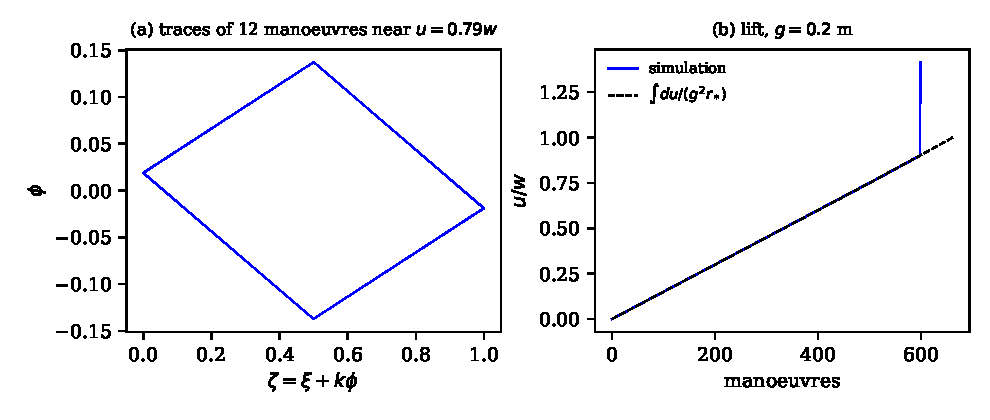
\includegraphics[width=\textwidth]{figures/fig_crawl.pdf}
\caption{The tilted crawl simulated with exact geometry, typical car, $g=0.2$ m.
(a) Rescaled traces of twelve consecutive manoeuvres near $u=0.79w$; they follow the $\lambda=1$ tilted loop at that height (cf.\ \cref{fig:window}).
(b) The lift $u$ against the number of manoeuvres, compared with the prediction $\int_0^u\dd v/(g^2r_*(v))$.
The final jump is the escape, once large tilts become admissible near the top.}
\label{fig:crawl}
\end{figure}

\subsection{Proofs of \texorpdfstring{\cref{thm:mono,thm:asym}}{Theorems}}\label{sec:asym-proofs}

\begin{proof}[Proof of \cref{thm:asym}]
\Cref{prop:asym-lower,prop:asym-upper} give $g^2N(g)\to K^2$.
For the equivalent statement let $\varepsilon\in(0,K^2)$.
For $g\le g_\varepsilon$ we have $(K^2-\varepsilon)/g^2\le N(g)\le(K^2+\varepsilon)/g^2$.
Since $\Lmin(n)-\ell=\inf\{g:N(g)\le n\}$, for $n$ large this gives $\sqrt{(K^2-\varepsilon)/n}\le\Lmin(n)-\ell\le\sqrt{(K^2+\varepsilon)/n}$.
Finally, $K^2=2Rw+\frac4R\int_0^{w/2}(R^2-t^2)\dd t=4Rw-\frac{w^3}{6R}$.
\end{proof}

\begin{proof}[Proof of \cref{thm:mono}]
Monotonicity is \cref{lem:monoL}.
By \cref{prop:asym-lower} there is $g_1>0$ with $N(g)\ge K^2/(2g^2)$ for $g\le g_1$.
So for each $n$, $N(g)>n$ for all $g<\min(g_1,K/\sqrt{2n})$, i.e.\ $\Lmin(n)\ge\ell+\min(g_1,K/\sqrt{2n})>\ell$.
By \cref{prop:asym-upper}, $N(g)<\infty$ for small $g$, so $\Lmin(n)\to\ell$.
\end{proof}
